
\section{Appendix}
\begin{table}[!htbp]
\footnotesize
\caption{Random Intercept Logistic Regression Predicting Mask Reference}
    \centering
    \begin{tabular}{l*{2}{c}}
\toprule
                    &\multicolumn{1}{c}{(1)}&\multicolumn{1}{c}{(2)}\\
                    &\multicolumn{1}{c}{Mask picturing}&\multicolumn{1}{c}{Mask mentioning}\\
\midrule
Woman  &      -0.266         &      -0.599         \\
                    &     (0.246)         &     (0.627)         \\
Republican     &      -0.881\sym{***}&      -0.734         \\
                    &     (0.235)         &     (0.720)         \\
Woman $\times$ Republican&       0.112         &      -0.912         \\
                    &     (0.387)         &     (1.647)         \\
Rurality      &      -0.117         &      -0.400         \\
                    &     (0.086)         &     (0.271)         \\
Trump vote share             &      -0.024\sym{*}  &       0.129\sym{***}\\
                    &     (0.010)         &     (0.037)         \\
Video               &       0.812\sym{***}&       0.062         \\
                    &     (0.031)         &     (0.128)         \\
Video \& image         &       1.261\sym{***}&       0.107         \\
                    &     (0.041)         &     (0.200)         \\
TV                  &       1.811\sym{***}&      -0.414         \\
                    &     (0.061)         &     (0.364)         \\
Incumbent                   &       0.519\sym{**} &      -1.040         \\
                    &     (0.194)         &     (0.651)         \\
Open race                   &       0.231         &       0.117         \\
                    &     (0.266)         &     (0.797)         \\
Senate              &      -0.422         &       0.510         \\
                    &     (0.237)         &     (0.632)         \\
Competitiveness &      -0.150\sym{*}  &      -0.509\sym{*}  \\
                    &     (0.070)         &     (0.222)         \\

Constant            &      -0.974         &     -11.909\sym{***}\\
                    &     (0.502)         &     (2.083)         \\
\midrule
var(\_cons[candidate\_fecid])&       2.260\sym{***}&      12.322\sym{***}\\
                    &     (0.226)         &     (2.707)         \\
\midrule
Observations        &      102529         &      102529         \\
\bottomrule
\multicolumn{3}{l}{\footnotesize Standard errors in parentheses}\\
\multicolumn{3}{l}{\footnotesize \sym{*} \(p<0.05\), \sym{**} \(p<0.01\), \sym{***} \(p<0.001\)}\\
\end{tabular}

    \label{table:tab2}
\end{table}

\begin{table}[!htbp]
    \caption{Random Intercept Logistic Regression on Mask Picturing and Mask Mentioning}
    \footnotesize
   \centering
   \begin{tabular}{l*{4}{c}}
\toprule
                    &\multicolumn{1}{c}{(1)}&\multicolumn{1}{c}{(2)}&\multicolumn{1}{c}{(3)}&\multicolumn{1}{c}{(4)}\\
                    &\multicolumn{1}{c}{Pooled}&\multicolumn{1}{c}{Pooled}&\multicolumn{1}{c}{FB}&\multicolumn{1}{c}{TV}\\
\midrule
Woman  &      -0.256         &      -0.319         &      -0.383         &      -0.082         \\
                    &     (0.249)         &     (0.240)         &     (0.267)         &     (0.255)         \\
Republican     &      -0.874\sym{***}&      -1.107\sym{***}&      -1.235\sym{***}&      -0.681\sym{**} \\
                    &     (0.238)         &     (0.229)         &     (0.257)         &     (0.244)         \\
Woman $\times$ Republican&       0.122         &       0.116         &       0.226         &      -0.450         \\
                    &     (0.392)         &     (0.378)         &     (0.423)         &     (0.409)         \\
Rurality      &      -0.130         &      -0.151         &      -0.146         &      -0.175         \\
                    &     (0.087)         &     (0.084)         &     (0.094)         &     (0.091)         \\
Trump vote share              &      -0.019         &      -0.012         &      -0.011         &      -0.016         \\
                    &     (0.010)         &     (0.010)         &     (0.011)         &     (0.012)         \\
Video              &       0.761\sym{***}&       0.580\sym{***}&       0.574\sym{***}&                     \\
                    &     (0.030)         &     (0.032)         &     (0.032)         &                     \\
Video,image         &       1.216\sym{***}&       0.902\sym{***}&       0.896\sym{***}&                     \\
                    &     (0.040)         &     (0.042)         &     (0.042)         &                     \\
TV                  &       1.795\sym{***}&       0.969\sym{***}&                     &                     \\
                    &     (0.061)         &     (0.062)         &                     &                     \\
Incumbent                   &       0.518\sym{**} &       0.370         &       0.268         &       0.565\sym{**} \\
                    &     (0.197)         &     (0.190)         &     (0.212)         &     (0.203)         \\
Open race                   &       0.261         &      -0.016         &      -0.042         &       0.115         \\
                    &     (0.269)         &     (0.260)         &     (0.291)         &     (0.289)         \\
Senate              &      -0.390         &      -0.181         &      -0.116         &      -0.268         \\
                    &     (0.240)         &     (0.231)         &     (0.258)         &     (0.228)         \\
Competitiveness &      -0.175\sym{*}  &      -0.116         &      -0.119         &      -0.127         \\
                    &     (0.071)         &     (0.069)         &     (0.077)         &     (0.071)         \\
Goal\_donate              &                     &      -2.203\sym{***}&      -2.224\sym{***}&       0.000         \\
                    &                     &     (0.036)         &     (0.037)         &         (.)         \\
Goal\_GOTV                &                     &      -2.426\sym{***}&      -2.436\sym{***}&                     \\
                    &                     &     (0.110)         &     (0.111)         &                     \\
Goal\_learnmore           &                     &      -0.679\sym{***}&      -0.694\sym{***}&      -0.163         \\
                    &                     &     (0.049)         &     (0.050)         &     (0.381)         \\
Goal\_other               &                     &      -3.881\sym{***}&      -3.894\sym{***}&       0.000         \\
                    &                     &     (0.137)         &     (0.137)         &         (.)         \\
Tone\_contrast            &                     &       0.440\sym{***}&       0.496\sym{***}&      -0.634         \\
                    &                     &     (0.064)         &     (0.066)         &     (0.336)         \\
Tone\_support             &                     &       0.710\sym{***}&       0.739\sym{***}&      -0.026         \\
                    &                     &     (0.060)         &     (0.061)         &     (0.334)         \\
Constant            &      -1.066\sym{*}  &      -0.888         &      -0.960         &       1.603\sym{*}  \\
                    &     (0.508)         &     (0.494)         &     (0.554)         &     (0.652)         \\
\midrule
var(\_cons[candidate\_fecid])&       2.342\sym{***}&       2.149\sym{***}&       2.630\sym{***}&       1.276\sym{***}\\
                    &     (0.232)         &     (0.215)         &     (0.284)         &     (0.258)         \\
\midrule
Observations        &      102529         &      102529         &      100551         &        1975         \\
\bottomrule
\multicolumn{5}{l}{\footnotesize Standard errors in parentheses}\\
\multicolumn{5}{l}{\footnotesize \sym{*} \(p<0.05\), \sym{**} \(p<0.01\), \sym{***} \(p<0.001\)}\\
\end{tabular}

\end{table}

\begin{table}[!htbp]
\title{Table A3: Random Intercept Logit on Mask Picturing and Mask Mentioning}
\footnotesize
    %\caption{Random Intercept Logistic Regression on Mask Picturing and Mask Mentioning}
   \centering
   \begin{tabular}{l*{2}{c}}
\toprule
                    &\multicolumn{1}{c}{(1)}&\multicolumn{1}{c}{(2)}\\
                    &\multicolumn{1}{c}{Mask picturing}&\multicolumn{1}{c}{Mask mentioning}\\
\midrule
Woman  &      -0.329         &      -0.602         \\
                    &     (0.239)         &     (0.619)         \\
Republican     &      -1.116\sym{***}&      -1.063         \\
                    &     (0.228)         &     (0.711)         \\
Woman $\times$ Republican&       0.101         &      -0.819         \\
                    &     (0.377)         &     (1.507)         \\
Rurality      &      -0.138         &      -0.398         \\
                    &     (0.083)         &     (0.268)         \\
Trump vote share              &      -0.018         &       0.133\sym{***}\\
                    &     (0.010)         &     (0.035)         \\
Video              &       0.628\sym{***}&       0.207         \\
                    &     (0.032)         &     (0.132)         \\
Video \& image         &       0.946\sym{***}&       0.310         \\
                    &     (0.042)         &     (0.205)         \\
TV                  &       0.981\sym{***}&      -0.830\sym{*}  \\
                    &     (0.062)         &     (0.354)         \\
Incumbent                   &       0.373\sym{*}  &      -1.182         \\
                    &     (0.189)         &     (0.633)         \\
Open race                   &      -0.051         &      -0.034         \\
                    &     (0.259)         &     (0.782)         \\
Senate              &      -0.210         &       0.676         \\
                    &     (0.230)         &     (0.621)         \\
Competitiveness &      -0.089         &      -0.466\sym{*}  \\
                    &     (0.068)         &     (0.215)         \\
Goal\_donate             &      -2.222\sym{***}&      -1.761\sym{***}\\
                    &     (0.037)         &     (0.182)         \\
Goal\_GOTV                &      -2.440\sym{***}&      -2.489\sym{***}\\
                    &     (0.112)         &     (0.731)         \\
Goal\_learnmore           &      -0.667\sym{***}&      -0.451         \\
                    &     (0.049)         &     (0.266)         \\
Goal\_other               &      -4.768\sym{***}&       1.004\sym{***}\\
                    &     (0.202)         &     (0.243)         \\
Tone\_contrast            &       0.472\sym{***}&      -1.129\sym{***}\\
                    &     (0.065)         &     (0.224)         \\
Tone\_support             &       0.750\sym{***}&      -0.819\sym{***}\\
                    &     (0.060)         &     (0.203)         \\

Constant            &      -0.821         &     -10.528\sym{***}\\
                    &     (0.493)         &     (1.970)         \\
\midrule
var(\_cons[candidate\_fecid])&       2.116\sym{***}&      10.425\sym{***}\\
                    &     (0.213)         &     (2.347)         \\
\midrule
Observations        &      102529         &      102529         \\
\bottomrule
\multicolumn{3}{l}{\footnotesize Standard errors in parentheses}\\
\multicolumn{3}{l}{\footnotesize \sym{*} \(p<0.05\), \sym{**} \(p<0.01\), \sym{***} \(p<0.001\)}\\
\end{tabular}

\end{table}

\begin{table}[!htbp]
%\textbf{\small{Table B: Random Intercept Logistic Regression on \\ Mask Picturing with Additional Controls}}
\title{Table A4: Random Intercept Logistic Regression on \\ Mask Picturing with Additional Controls}
\footnotesize
    %\caption{Random Intercept Logistic Regression on Mask Picturing and Mask Mentioning}
   \centering
   \begin{tabular}{l*{3}{c}}
\toprule
                    &\multicolumn{1}{c}{(1)}&\multicolumn{1}{c}{(2)}&\multicolumn{1}{c}{(3)}\\
                    &\multicolumn{1}{c}{Mask\_picturing}&\multicolumn{1}{c}{Mask\_picturing}&\multicolumn{1}{c}{Mask\_picturing}\\
\midrule
Woman &       0.275         &       0.148         &       0.154         \\
                    &     (0.447)         &     (0.456)         &     (0.454)         \\
Republican    &      -0.528         &      -0.900\sym{*}  &      -0.970\sym{*}  \\
                    &     (0.445)         &     (0.454)         &     (0.453)         \\
Woman $\times$ Republican&      -0.022         &       0.204         &       0.237         \\
                    &     (0.730)         &     (0.742)         &     (0.741)         \\
Rurality      &      -0.161         &      -0.236         &      -0.232         \\
                    &     (0.164)         &     (0.167)         &     (0.166)         \\
Incumbent                   &       0.641         &       0.707         &       0.678         \\
                    &     (0.362)         &     (0.369)         &     (0.368)         \\
Open race                   &       0.038         &      -0.383         &      -0.480         \\
                    &     (0.518)         &     (0.533)         &     (0.532)         \\
Senate              &       0.681         &       0.883\sym{*}  &       0.840         \\
                    &     (0.439)         &     (0.447)         &     (0.445)         \\
Competitiveness &      -0.404\sym{**} &      -0.287\sym{*}  &      -0.279\sym{*}  \\
                    &     (0.132)         &     (0.134)         &     (0.133)         \\
Trump vote share              &      -0.012         &      -0.004         &      -0.003         \\
                    &     (0.020)         &     (0.020)         &     (0.020)         \\
Goal\_donate              &                     &      -1.923\sym{***}&      -1.908\sym{***}\\
                    &                     &     (0.078)         &     (0.079)         \\
Goal\_GOTV                &                     &      -1.650\sym{***}&      -1.492\sym{***}\\
                    &                     &     (0.198)         &     (0.199)         \\
Goal\_Learnmore           &                     &      -2.748\sym{***}&      -2.713\sym{***}\\
                    &                     &     (0.164)         &     (0.165)         \\
Goal\_Other               &                     &      -4.716\sym{***}&      -4.553\sym{***}\\
                    &                     &     (0.240)         &     (0.240)         \\
Tone\_contrast            &                     &       0.732\sym{***}&       0.629\sym{***}\\
                    &                     &     (0.179)         &     (0.180)         \\
Tone\_support             &                     &       0.605\sym{***}&       0.599\sym{***}\\
                    &                     &     (0.165)         &     (0.166)         \\
No. of face          &                     &                     &       0.100\sym{***}\\
                    &                     &                     &     (0.007)         \\
Constant            &      -3.182\sym{***}&      -3.055\sym{**} &      -3.280\sym{***}\\
                    &     (0.954)         &     (0.989)         &     (0.986)         \\
\midrule
/                   &                     &                     &                     \\
var(\_cons[candidate\_fecid])&       5.837\sym{***}&       5.931\sym{***}&       5.784\sym{***}\\
                    &     (0.973)         &     (0.994)         &     (0.970)         \\
\midrule
Observations        &       47668         &       47668         &       47668         \\
\bottomrule
\multicolumn{4}{l}{\footnotesize Standard errors in parentheses}\\
\multicolumn{4}{l}{\footnotesize \sym{*} \(p<0.05\), \sym{**} \(p<0.01\), \sym{***} \(p<0.001\)}\\
\end{tabular}

\end{table}
\clearpage


\clearpage
\section{Fightin' Words}
\begin{figure}[!htbp] % specifier
    \caption{Fightin words z-scores by party. Words with higher values (positive or negative) are more associated with a specific party.}
    \centering % The default alignment is left.
    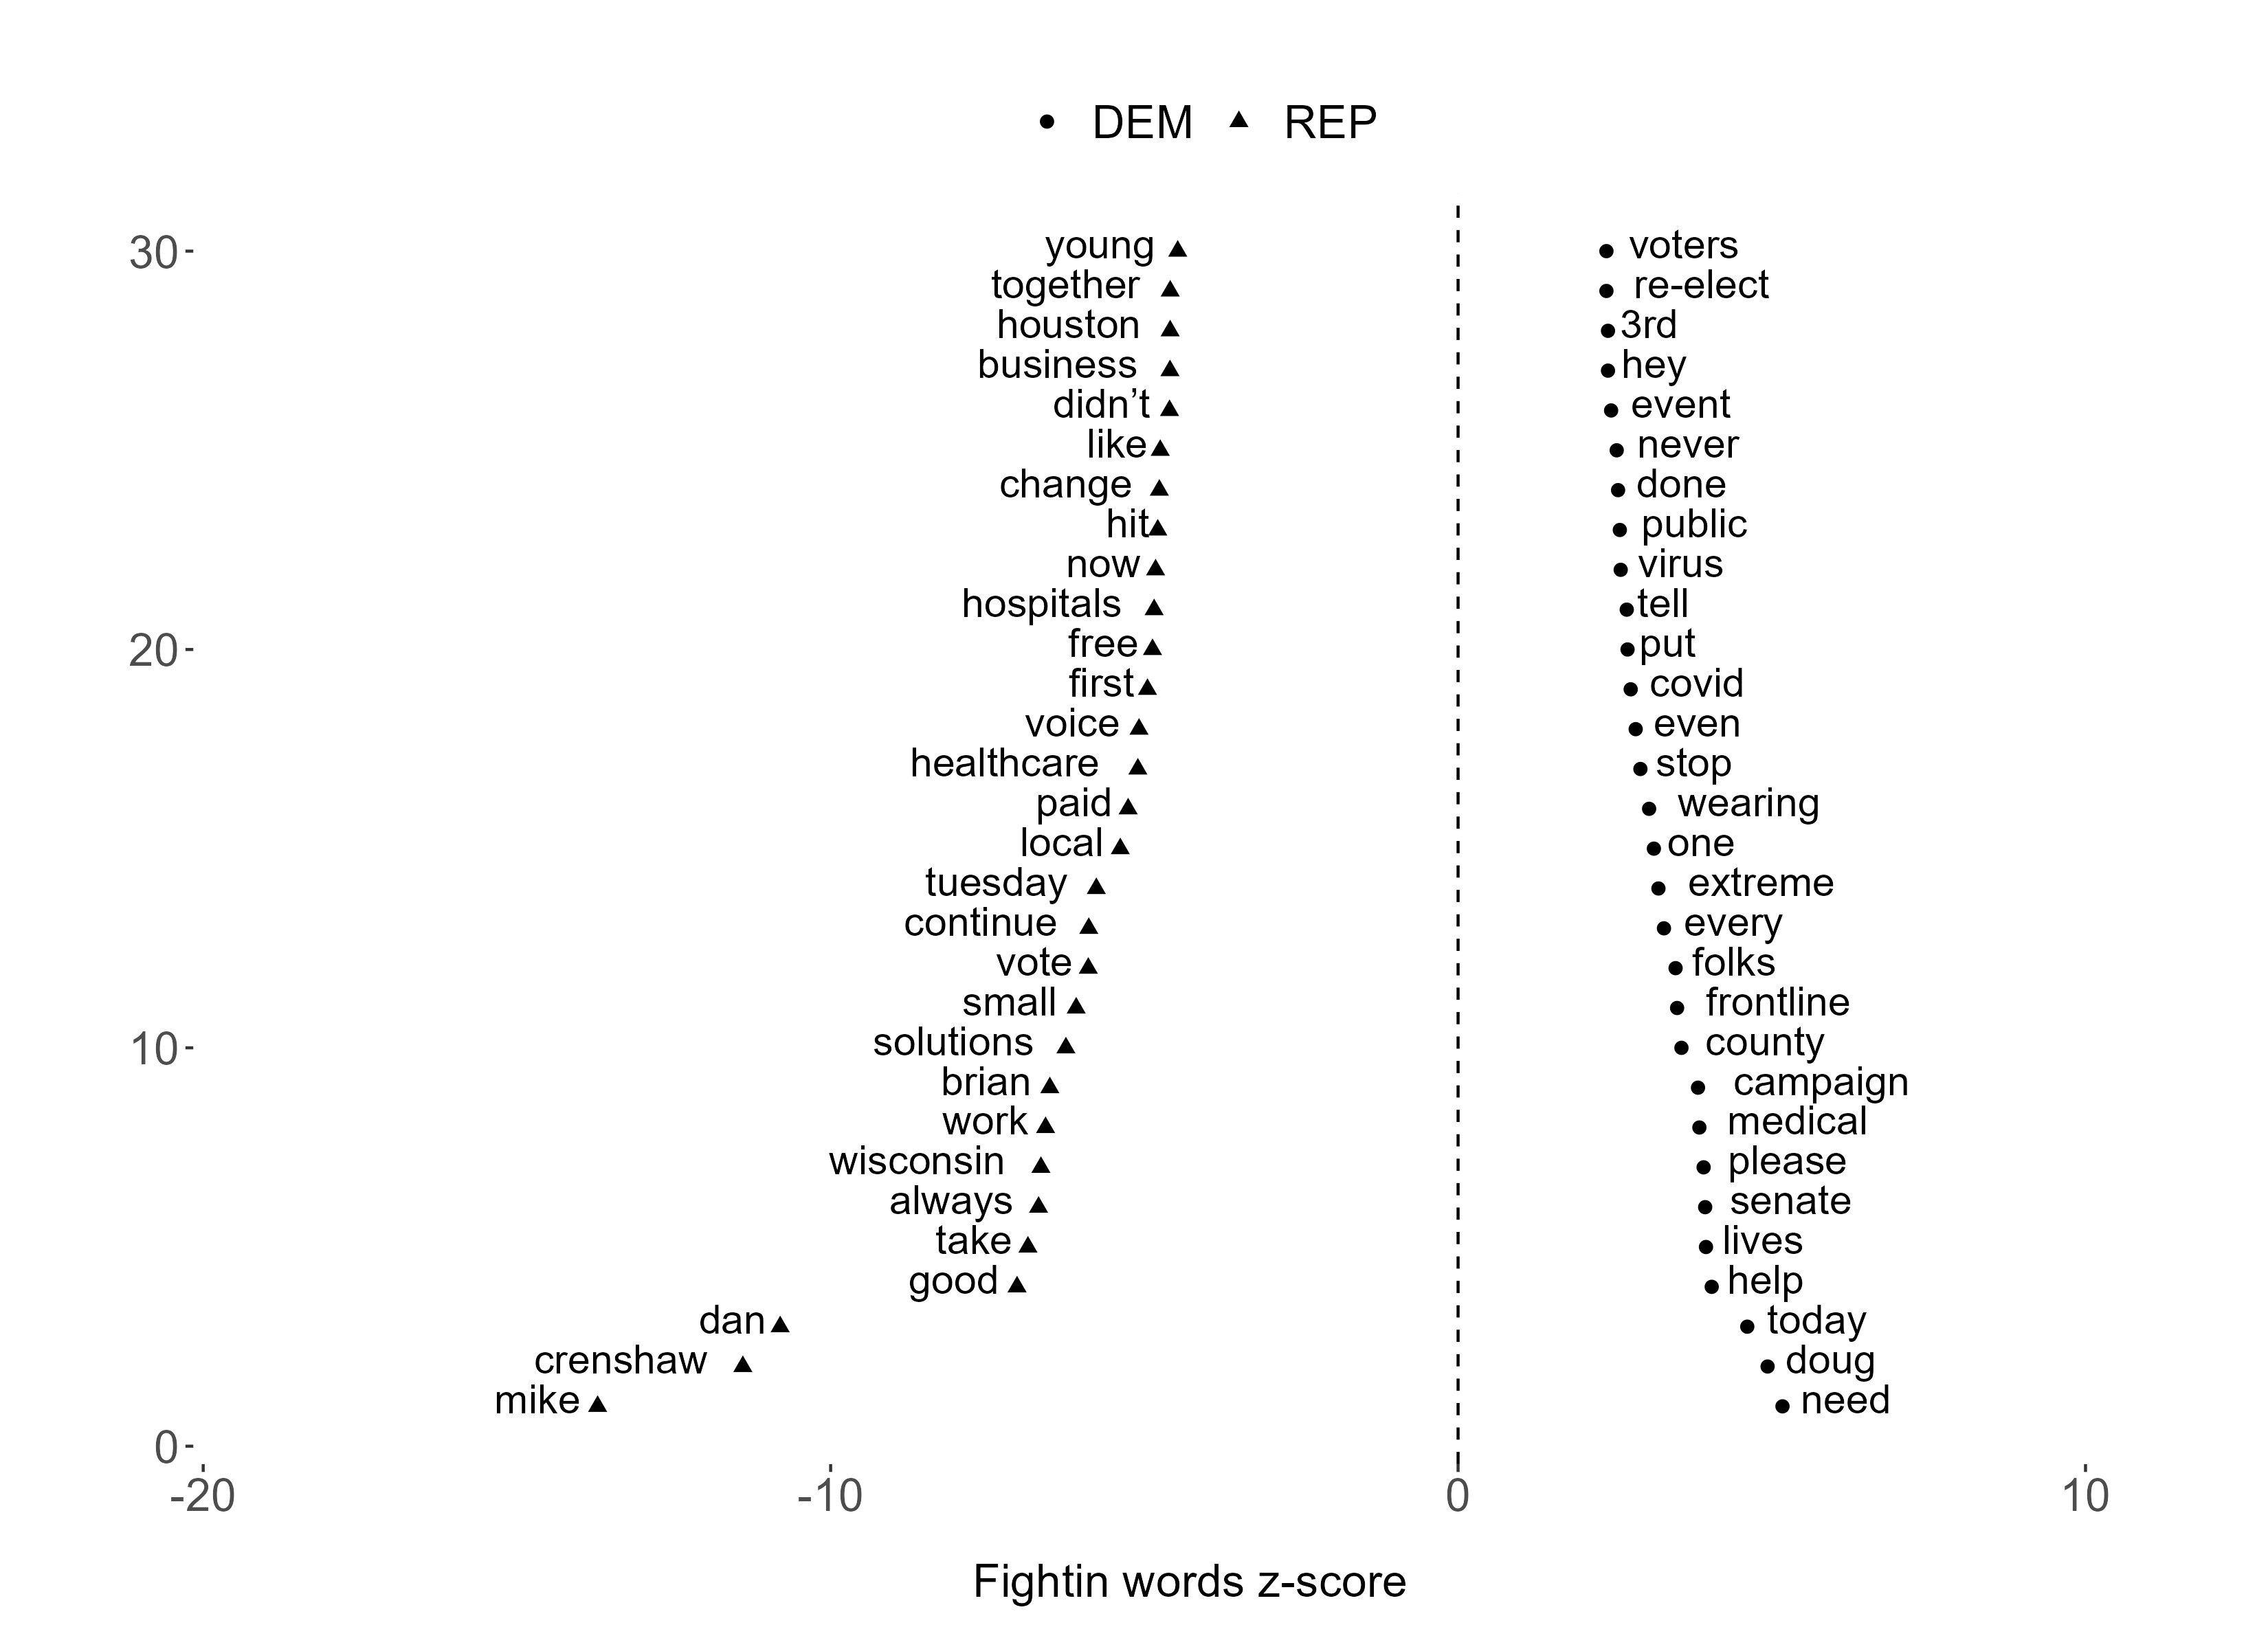
\includegraphics[width = 0.8\textwidth]{fw_party.png}.
    \label{fig:fw_party}
\end{figure}

\begin{figure}[!htbp] % specifier
    \caption{Fightin words z-scores by gender. Words with higher values (positive or negative) are more associated with a specific gender.}
    \centering % The default alignment is left.
    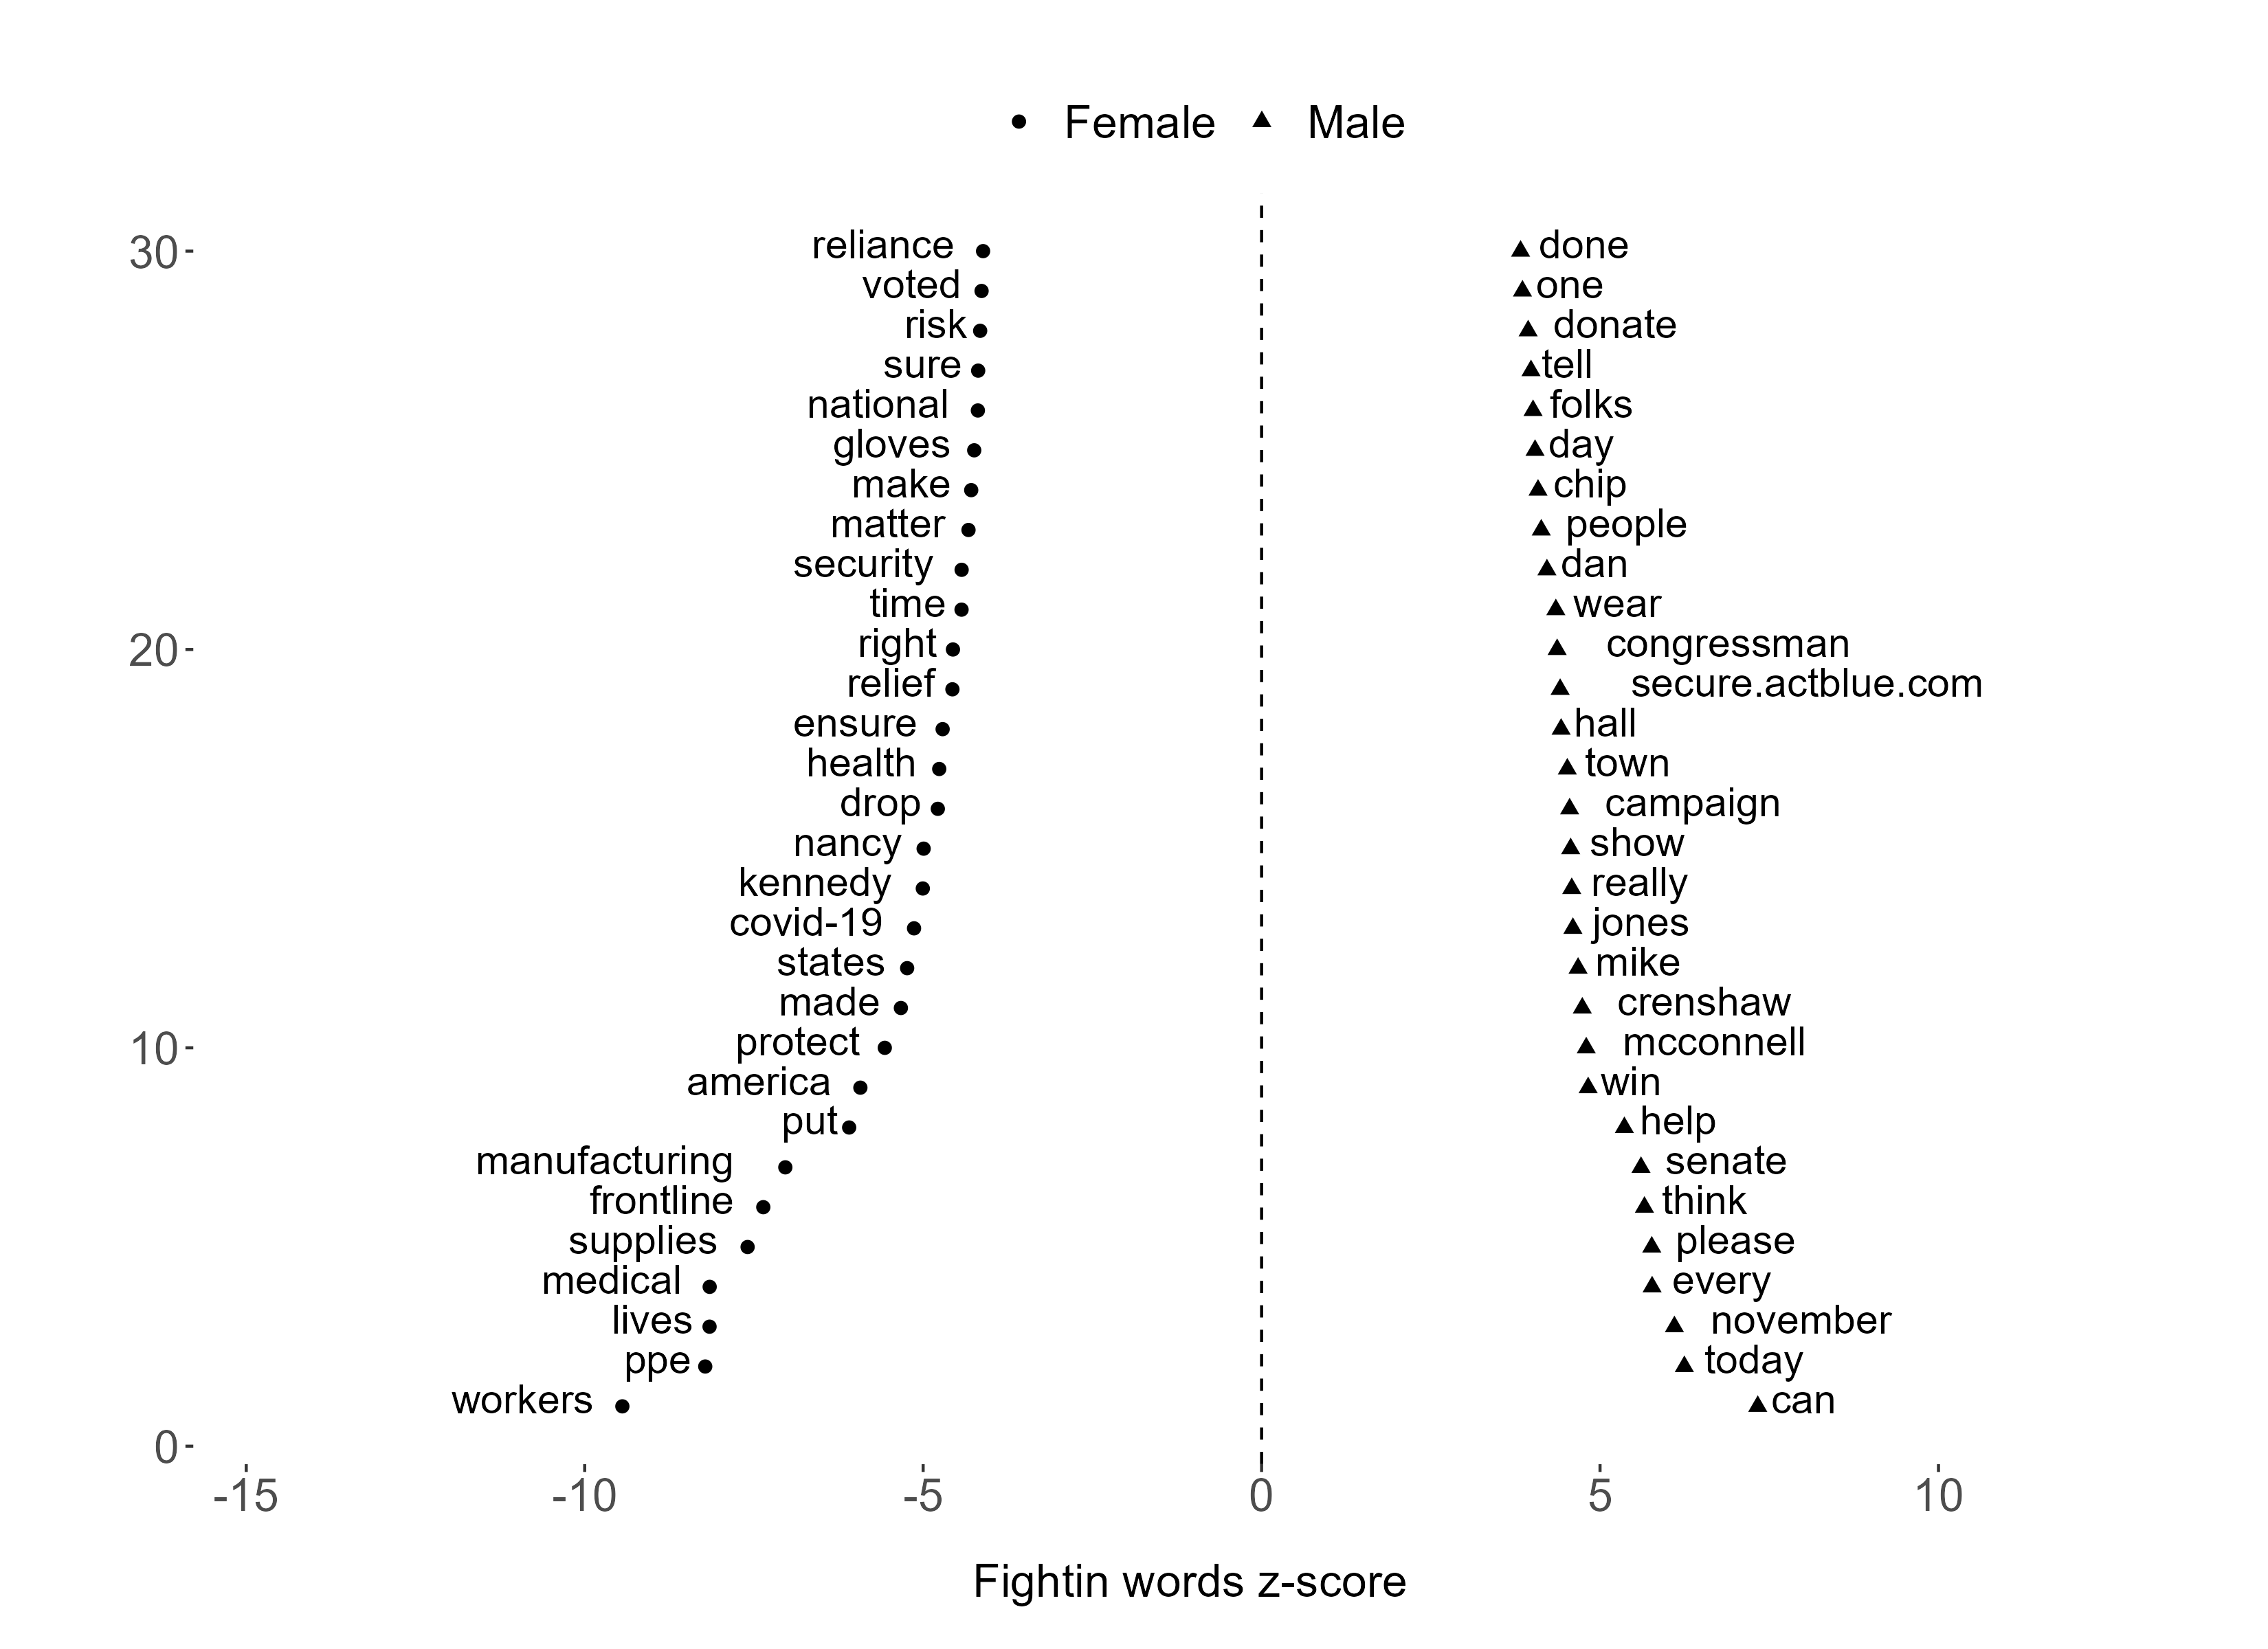
\includegraphics[width = 0.8\textwidth]{fw_gender.png}.
    \label{fig:fw_gender}
\end{figure}


\clearpage
\section{Structural Topic Models}
\begin{figure}[!ht] % specifier
    \caption{Structural topic model - difference in topic proportions between Democrats and Republicans. Topics with higher values are more associated with Democrats. The words to the left of the estimate are the top words of the topic.}
    \centering % The default alignment is left.
    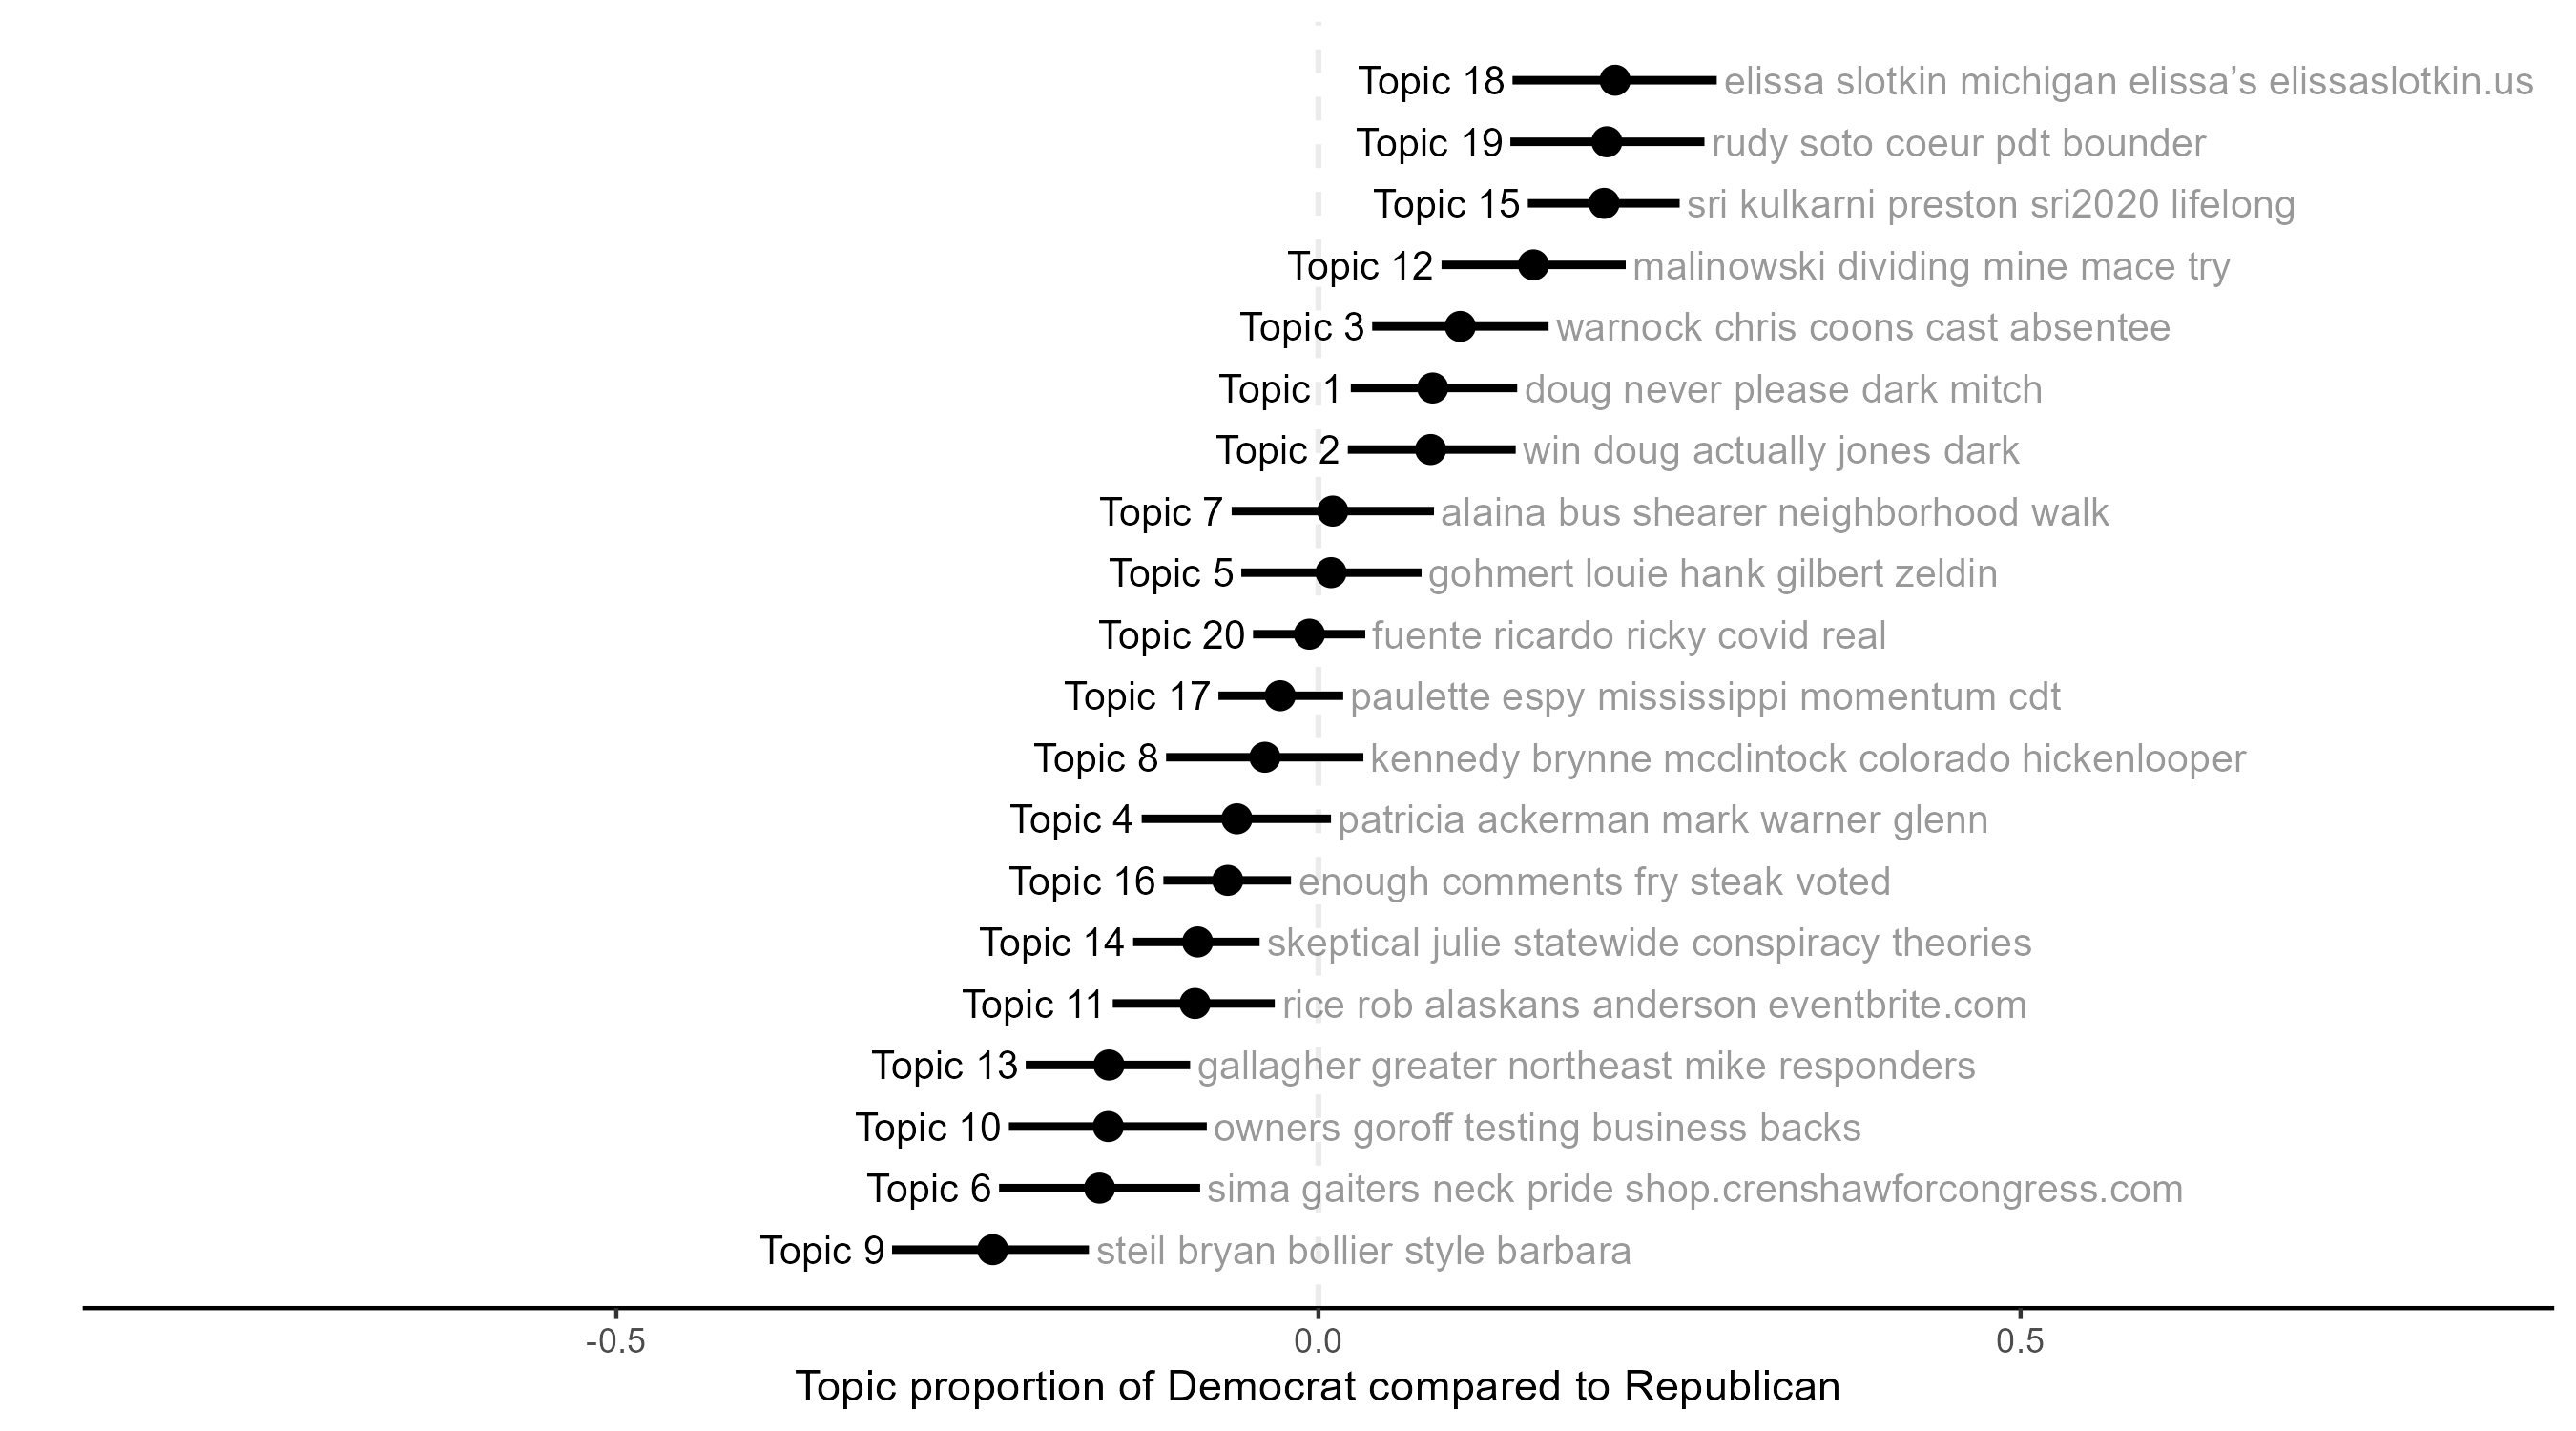
\includegraphics[width = \textwidth]{democratic_topics.png}
    \label{fig:stm_party}
\end{figure}

\begin{figure}[!htbp] % specifier
    \caption{Structural topic model - difference in topic proportions between women and men candidates. Topics with higher values are more associated with women candidates. The words to the left of the estimate are the top words of the topic.}
    \centering % The default alignment is left.
    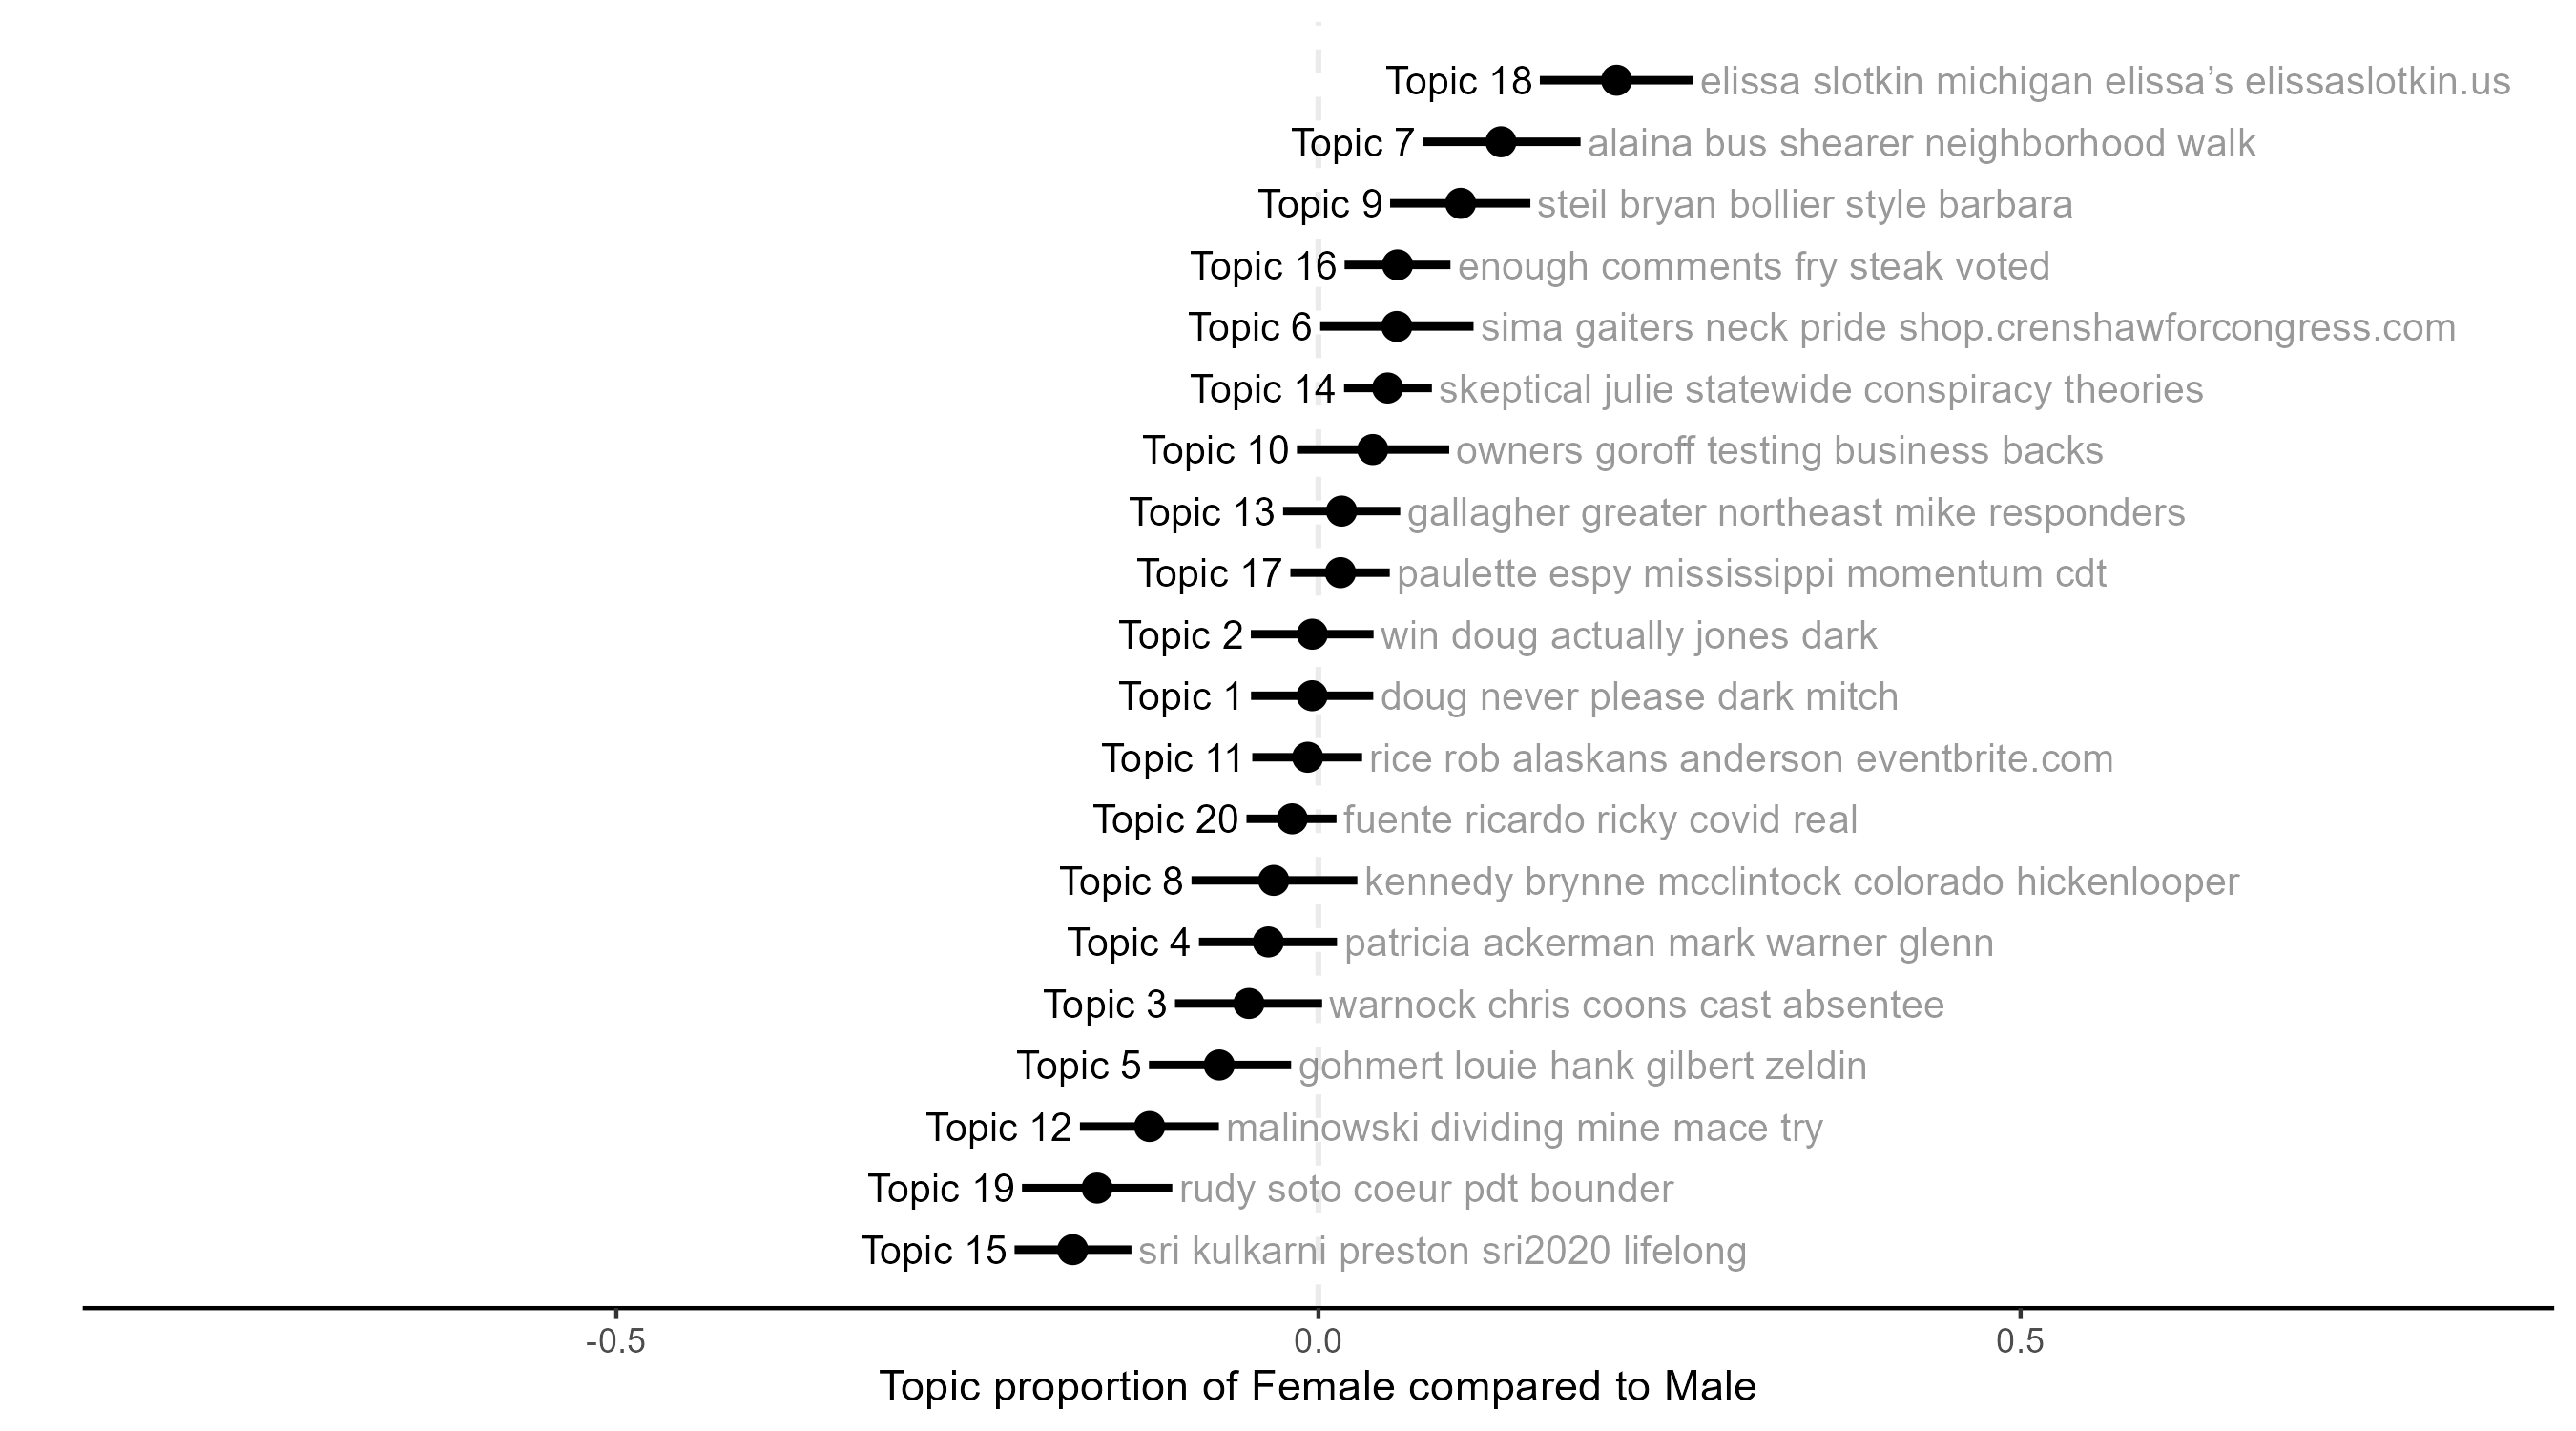
\includegraphics[width = \textwidth]{female_topics.png}
    \label{fig:stm_gender}
\end{figure}